%----------------------------------------------------------------------------------------
%	PACKAGES AND DOCUMENT CONFIGURATIONS
%----------------------------------------------------------------------------------------

\documentclass[11pt]{article}

\usepackage{graphicx} % Required for the inclusion of images
\usepackage{natbib} % Required to change bibliography style to APA
\usepackage{amsmath} % Required for some math elements 
\usepackage{subcaption}
\usepackage[justification=centering]{caption}
\usepackage[nomarkers,figuresonly]{endfloat}
\usepackage[margin=0.9in]{geometry}
\usepackage{sectsty}
\sectionfont{\fontsize{12}{15}\selectfont}
\setlength\parindent{0pt} % Removes all indentation from paragraphs

\renewcommand{\labelenumi}{\alph{enumi}.} % Make numbering in the enumerate environment by letter rather than number

%%%%%%%%%% Start TeXmacs macros
\newcommand{\nocomma}{}
\newcommand{\noplus}{}
\newcommand{\tmop}[1]{\ensuremath{\operatorname{#1}}}
\newcommand{\upl}{+}
%%%%%%%%%% End TeXmacs macros

%----------------------------------------------------------------------------------------
%	DOCUMENT INFORMATION
%----------------------------------------------------------------------------------------

\title{Machine Translation Assignment 2: Decoding} % Title

\author{s0907677, s1520582} % Author name

\date{}

\begin{document}

\maketitle % Insert the title, author and date

%----------------------------------------------------------------------------------------
%	Q 1
%----------------------------------------------------------------------------------------
\section*{Q1}
The default limitation of both stack size and maximum number of translation to 1 is very restrictive and so one expects to see a significant improvement in total log probability once either limit is increased. This proves to be true, but only in a very limited range for both variables.

Changing the maximum number of translations from 1 to 2 leads to a relatively sharp improvement, which flattens out very quickly. The difference in total log probability between decoder with k=10 and k=50 is only 10\% of the difference between k=1 and k=2. No further improvements are observed for k>50.

Changing the stack size has a similar effect, although improvement tapers out even quicker. Increasing stack size to over 3 does not provide significant benefits.

Qualitatively, the difference between translations produced by the maximally limited system (k=1 and s=1) and one which produces the highest scoring output (k=50 and s=10) is that the latter text is more fluent and idiomatic,  yet the meaning is equally difficult to grasp and there is no difference between the levels of syntactic correctness.

We did not investigate how parameter changes affect decoding speed. Simple timing methods seemed to be neither sensitive nor reliable enough to uncover any interesting trends for values of k and s in the range [1-100]. We did not investigate higher values because they did not offer improvement in total log probability.

The conclusions to draw from these results are:
(a) the intuitive insight that phrases can have multiple good translations proves to be important. Increasing the maximum number of possible translations per phrase does improve output quality.
(b) the pruning heuristics used in decoding are justifiable, since the best translation really can be found by searching within the top few hypothesis in each stack. The best hypothesis is not always the very top one, as witnessed by the sharp increase in log probability when stack size is changed to 2, but it seems to almost always be one of the top 5 or so hypothesis.
(c) there is a limit, and one that's quickly reached, to how good a monotonic decoder can be. Allowing it to entertain more possible translations cannot overcome inherent problems entailed by monotonicity.

\begin{figure}
	\centering
	\begin{subfigure}{.8\linewidth}
		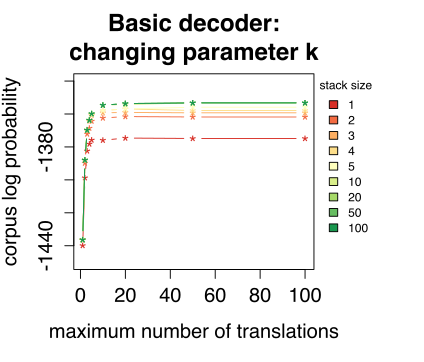
\includegraphics[scale=.75]{d1_k.png}
		\caption{Increasing maximum number of translations, range [1-100].}
	\end{subfigure}
	\hskip2em
	\begin{subfigure}{.8\linewidth}
		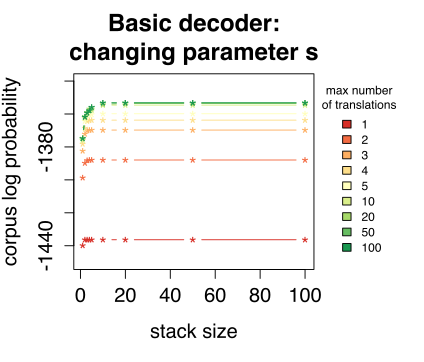
\includegraphics[scale=.75]{d1_s.png}
		\caption{Increasing stack size, range [1-100].}
	\end{subfigure}
	\caption{Performance of decoder without reordering.}
\end{figure}

%----------------------------------------------------------------------------------------
%	Q 2
%----------------------------------------------------------------------------------------
\section*{Q2}
We modified the old $h(j,e)$ so that each recursion step reads two French phrases
instead of one. The second of these phrases may be either an actual phrase or an artificial  empty phrase $\varepsilon$, which we have added to the translation dictionary. The $\varepsilon$ phrase is an empty string, which translates with probability one to an empty string. The two read phrases are always swapped in the translation. In case of the second phrase being $\varepsilon$, the swapping is only nominal and the resulting translation is as if no swapping was performed.
Our full definition of $h(j,e)$ is specified as follows:

$h (0 \nocomma, e) = \left\{ \begin{array}{l}
1 \nocomma, \tmop{if} \, e = \tmop{START}\\
0 \nocomma, \tmop{otherwise}
\end{array} \right.$
\begin{eqnarray}
h (j, e) = & \underset{h (i, e') e_1 \ldots e_k e_{k + 1} \ldots e_m
	e}{\tmop{argmax}}_{} & p (h (i, e')) \nonumber\\
& + & \log p_{\tmop{TM}} (f_{i + 1} \ldots f_c |e_{k + 1} \ldots e_m e)
\nonumber\\
& \noplus + & \log p_{\tmop{TM}} (f_{c + 1} \ldots f_j |e_1 \ldots e_k)
\nonumber\\
& \upl & \log p_{\tmop{LM}} (e_1 |e') + \sum_{k' = 1}^{m - 1} \log
p_{\tmop{LM}} (e_{k' + 1} |e_{k'}) + \log p_{\tmop{LM}} (e|e_m) \nonumber
\end{eqnarray}
with $0 \leq i < c \leq j$, $0 \leq k \leq m$, $e' \in V_E$, $e_1 \ldots e_k
\in t (f_{c + 1} \ldots f_j) \cup \{ \varepsilon \}$,\\
and $e_{k + 1} \ldots e_m e \in t (f_{i + 1} \ldots f_c)$.



%----------------------------------------------------------------------------------------
%	Q 3
%----------------------------------------------------------------------------------------
\section*{Q3}
For each French sentence of length $n$, we loop over all $n$ possible stacks. In each stack, we look at the top $s$ hypotheses and expand them. To perform an expansion we choose two consecutive phrases (the second of which might be $\varepsilon$), swap them, and consider all possible combinations of the first $k$ translations of each phrase. The maximum considered length of phrase is $n$. Finally, the algorithm calculates the language model probability of the generated two-phrase translation. In this step, the algorithm has to iterate over up to $2 t$ words, where $t$ is the maximum length of a translation phrase. Thus the overall complexity is as follows:

\[
\mathcal{O}(n \cdot s) \cdot \mathcal{O}({(n \cdot k)}^2)
\cdot \mathcal{O}(t)
= \mathcal{O}(n^3 \cdot k^2 \cdot s \cdot t)
\]

%----------------------------------------------------------------------------------------
%	Q 4
%----------------------------------------------------------------------------------------
\section*{Q4}
In our implementation the mapping from hypotheses to stacks is the same in the decoder with local reordering as it was in the one without. Each hypothesis is placed on a stack corresponding to the index of last French word being translated. We do not create hypotheses in which French phrases are skipped, but instead always look at two consecutive phrases, swap then, and create a hypothesis which covers both phrases. This means that mapping onto stacks is straightforward, since the number of French words covered by a hypothesis is always the same as the index of the last word which it translates.

%----------------------------------------------------------------------------------------
%	Q 5
%----------------------------------------------------------------------------------------
\section*{Q5}
Our implementation of local reordering does not involve any changes to the hypotheses objects. We do modify the translation model by inserting into the dictionary an empty phrase, which translates to English with probability 1 as an empty string.

We introduce a modification in the hypothesis extension step. Given a hypothesis which ends at index \textit{i} in the French sentence we consider all indices \textit{c} and \textit{j} such that $c \leq j$, $j \leq sentence length$, and the fragments of the sentence delimited by \textit{[i, c]} and \textit{[c, j]} are phrases. Since we allow for $c = j$, the second phrase may be the empty one we have added to the translation model. For each discovered pair of phrases we create a hypothesis by swapping them and considering k best translations for each. For a pair with an empty phrase this amounts to no reordering. The hypotheses we generate do not have gaps in coverage of the source sentence and can be simply placed on the stack corresponding to the last word covered.

This approach provides for a simple implementation. We do not need to check if the hypothesis we are extending was or was not created by skipping a phrase. Each hypothesis we store was either created by reordering the last two phrases it covers, or by translating monotonically. In both cases we are free to reorder any next two consecutive phrases we find in the French sentence.

%----------------------------------------------------------------------------------------
%	Q 6
%----------------------------------------------------------------------------------------
\section*{Q6}

The effects of k and s on speed are much more noticeable that for the simple decoder.

\begin{figure}
	\centering
	\begin{subfigure}{.8\linewidth}
		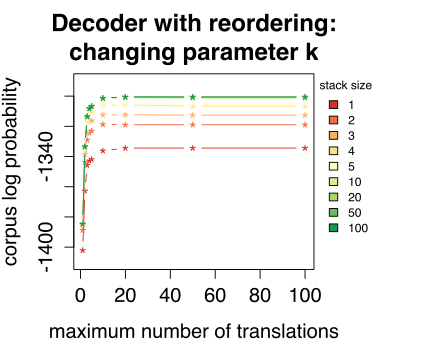
\includegraphics[scale=.75]{d2_k.png}
		\caption{Increasing maximum number of translations, range [1-100].}
	\end{subfigure}
	\hskip2em
	\begin{subfigure}{.8\linewidth}
		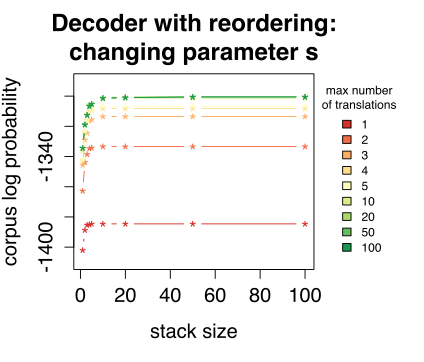
\includegraphics[scale=.75]{d2_s.png}
		\caption{Increasing stack size, range [1-100].}
	\end{subfigure}
	\caption{Performance of decoder with local reordering.}
\end{figure}

\begin{figure}
	\centering
	\begin{subfigure}{.45\linewidth}
		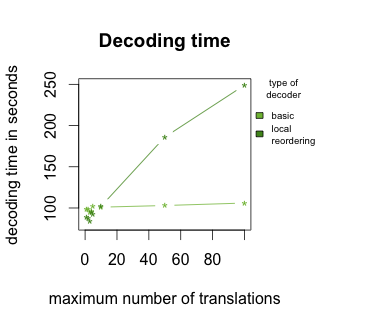
\includegraphics[scale=.55]{k_time.png}
		\caption{Decoding time as function of maximum number of translations.}
	\end{subfigure}
	\hskip2em
	\begin{subfigure}{.45\linewidth}
		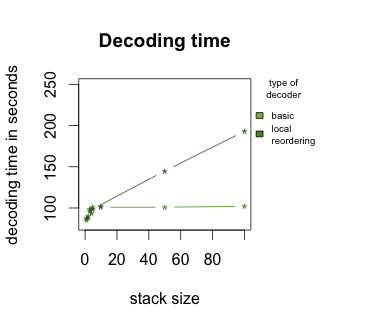
\includegraphics[scale=.55]{s_time.png}
		\caption{Decoding time as a function of stack size.}
	\end{subfigure}
	\caption{Decoding time for the basic decoder and decoder with reordering.}
\end{figure}

%----------------------------------------------------------------------------------------
%	Q 7
%----------------------------------------------------------------------------------------
\section*{Q7}
We based our decoder on the correspondence between phrase-based decoding and the Traveling Salesmen Problem, following the proposal of \cite{zaslavskiy2009}.

Our implementation includes the following steps:
- create an asymmetric graph based on the French sentence, the translation model, and the English model;
- find the best path by utilizing the LKH package implementation of the Lin-Kernighan heuristic \cite{Helsgaun2006};

We transform a sentence into a asymmetric graph by following the procedure described in \cite{zaslavskiy2009}. We extract from the French sentence all phrases; for each phrase we retrieve all of its possible translations and for each of these we create a biphrase (French phrase, English translation). Then we create nodes of the graph by generating all possible pairs of a French word taken from the sentence and a biphrase of which this word is a part. Having crated all the nodes, we decide on the cost of each possible directed edge, again following the approach described in the article. We do not transform our graph to a symmetric one, since the TSP solver we use is capable of handling problems specified as asymmetric graphs.

\begin{figure}
	\centering
	\begin{subfigure}{.8\linewidth}
		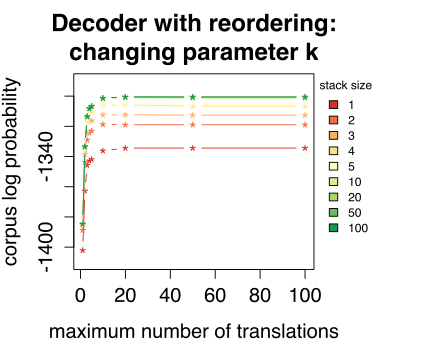
\includegraphics[scale=.75]{d2_k.png}
		\caption{Increasing maximum number of translations, range [1-100].}
	\end{subfigure}
	\hskip2em
	\begin{subfigure}{.8\linewidth}
		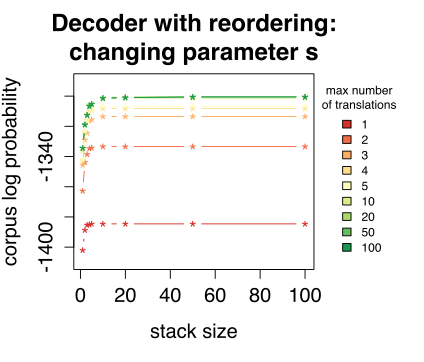
\includegraphics[scale=.75]{d2_s.png}
		\caption{Increasing stack size, range [1-100].}
	\end{subfigure}
	\caption{Performance of TSP-besed decoder.}
\end{figure}

%----------------------------------------------------------------------------------------
%	BIBLIOGRAPHY
%----------------------------------------------------------------------------------------
\bibliographystyle{apalike}

\bibliography{bibliography}

%----------------------------------------------------------------------------------------


\end{document}
